\documentclass[
class = book,
zihao = -4,
font = noto,
paper = a4paper,
openany
]{easybook}

\usepackage{xju}
\newcommand{\ti}{Ti6Al4V}

\begin{document}
	\hypersetup{pdftitle=Ti-6Al-4V 钛合金热处理工艺的研究现状及进展,pdfauthor=田欣洋,pdfsubject={材料科学,金属学,钛合金},pdfkeywords={热处理,固溶,时效,组织},pdfstartview=FitB}
	\maketitle
	\frontmatter*[roman]

	\begin{abstract}
		\ti 合金又名TC4合金,拥有较好的塑韧性、耐热性、成形性、耐蚀性等,
		%	其使用量已占钛合金使用总量的75$ \% $~85$ \% $,也是大多数高强钛合金的基础,被誉为钛合金中的“王牌合金”,
		在机械、军事、航空航天等领域获得了极为广泛的应用。但TC4合金仍存在硬度较低、摩擦磨损系数高、耐磨性能差、较低的塑韧性和力学性能上的各向异性等缺点,制约了其进一步的应用。本文旨在调研固溶时效处理Ti6Al4V合金强度的影响,并分析了不同固溶时效工艺参数下处理Ti6Al4V合金的力学性能,确定了最佳的固溶温度、时效温度、失效时间等参数,为工程应用提供了有价值的参考。
%		\begin{enumerate}
%			\item (\text{\color{blue}从热处理制度})在950℃进行固溶、550℃进行时效处理时可以得到合金最佳的力学性能。
%			\item (\text{\color{blue}从微观组织})冷却速率越高,得到组织所含$ \beta  $相含量越多,综合性能越好。
%			\item (\text{\color{blue}从转变机理})时效时间越久,亚稳定$ \beta $相分解的就越充分,得到的组织性能更好。
%		\end{enumerate}
\\

		\keywords{Ti-6Al-4V 钛合金;热处理;显微组织;力学性能;现状}
	\end{abstract}

	\tableofcontents
	\mainmatter*

	\pagestyle{Xju}
	\newcommand{\hot}[9]{
					#1 & #2 & $\mathrm{#3}$ & #4 & #5 & $\mathrm{#6}$ & #7& #8 & #9 &
%
%
%		固溶温度为#1 \textcelsius,
%
%		固溶时间为#2 h,
%
%		固溶处理冷却方式为#3;
%
%		时效温度为#4 \textcelsius,
%
%		时效时间为#5 h,
%
%		时效处理冷却方式为#6。#7
	}
	\chapter{前言}
Ti6Al4V合金具有较高的抗拉强度和抗疲劳强度、弹性模量低、低密度、高硬度和良好的耐腐蚀性能。

\section{参考甲}
\subsection{试样}
拉伸试样的尺寸参数:厚度是7毫米,宽度(20±0.05)毫米,长度(60 + 0.5)毫米。夹紧端是50毫米的长度。曲率之间的平行段长度和夹紧端是大于或等于12。拉伸试样的总长度大于184mm。应变 率 是 0.003 $ s^{-1} $。
\newpage
\subsection{机理}
%The α-phase is the substrate phase of (α+β)-titanium alloy. The number, shape and size of α-phase determine directly the property of (α+β)-titanium alloy. In the two-phase region, (α+β)-phase is gotten from the heat treatment with different holding time and temperatures. The temperature is below the phase transition temperature. The main characteristics of (α+β)-phase microstructure are irregular shape of grains, continuous and discontinuous α-phase on the grain boundary, and many small secondary α-phases. The punctate, spherical, flakiness and short rod α-phase exists in intragranular[22]. However, all (α+β)-phase will be converted into β-phase when the heating temperature is higher than phase transition temperature. The size and shape of grains are not identical. They are quadrilateral, pentagon and hexagon.
%
%Solution and aging can eliminate or reduce α-phase of continuous grain boundary. They can improve significantly the tensile and fatigue strength. But the plasticity will decrease a little. Solution and aging treatment can improve obviously the fatigue strength. The more stable β-phase of alloy, the more β-phase metastable after quenching. Then the effect of aging strengthening is better. Maximum effect will be gotten when the temperature of β stable element reaches CK value. Strengthening effect decreases with the rise of β-phase. That causes precipitation of aging β-phase metastable and the number of α-phase declines. Ti6Al4V alloy is (α+β)-phase alloy. The microstructure and mechanical properties can be improved by the solution and aging heat treatment, and then better comprehensive properties can be obtained [23,24].
	\begin{table}[htbp]
		\centering
		\label{sec:myHT}
		\caption{\ti 热处理工艺与性能汇总表\cite{LiuWanYingBuTongReChuLiGongYiDuiTi6Al4VTaiHeJinWeiGuanJieGouHeLiXueXingNengYingXiangYingWen2017}}
		\resizebox{\textwidth}{!}{
		\begin{tabular}{cccccc|cccc}
			\toprule
			固溶温度/℃ &用时/h & 冷却 & 时效温度/\textcelsius &用时/h & 冷却&屈强/Mpa&抗拉强度/Mpa&延伸率$\%  $&冲击韧性$ A_k /j \cdot cm^{-2} $ \\
			\midrule
			\hot{热轧}{——}{——}{——}{——}{——}{700}{790}{12.81}27.60\\
			\hot{920}{1}{WQ}{450}{4}{AC}{890}{1000}{15.00}40.00\\
			\hot{920}{1}{WQ}{500}{4}{AC}{960}{1070}{13.82}38.21\\
			\hot{960}{1}{WQ}{450}{4}{AC}{960}{1050}{15.48}43.64\\
			\hot{960}{1}{WQ}{500}{4}{AC}{1050}{1120}{16.28}46.22\\
			\hot{1000}{1}{WQ}{450}{4}{AC}{1000}{1100}{12.08}33.05\\			\hot{1000}{1}{WQ}{550}{4}{AC}{1020}{1100}{10.23}30.63\\
			\bottomrule
		\end{tabular}
	}
	\end{table}
\begin{figure}[h!]
	\centering
	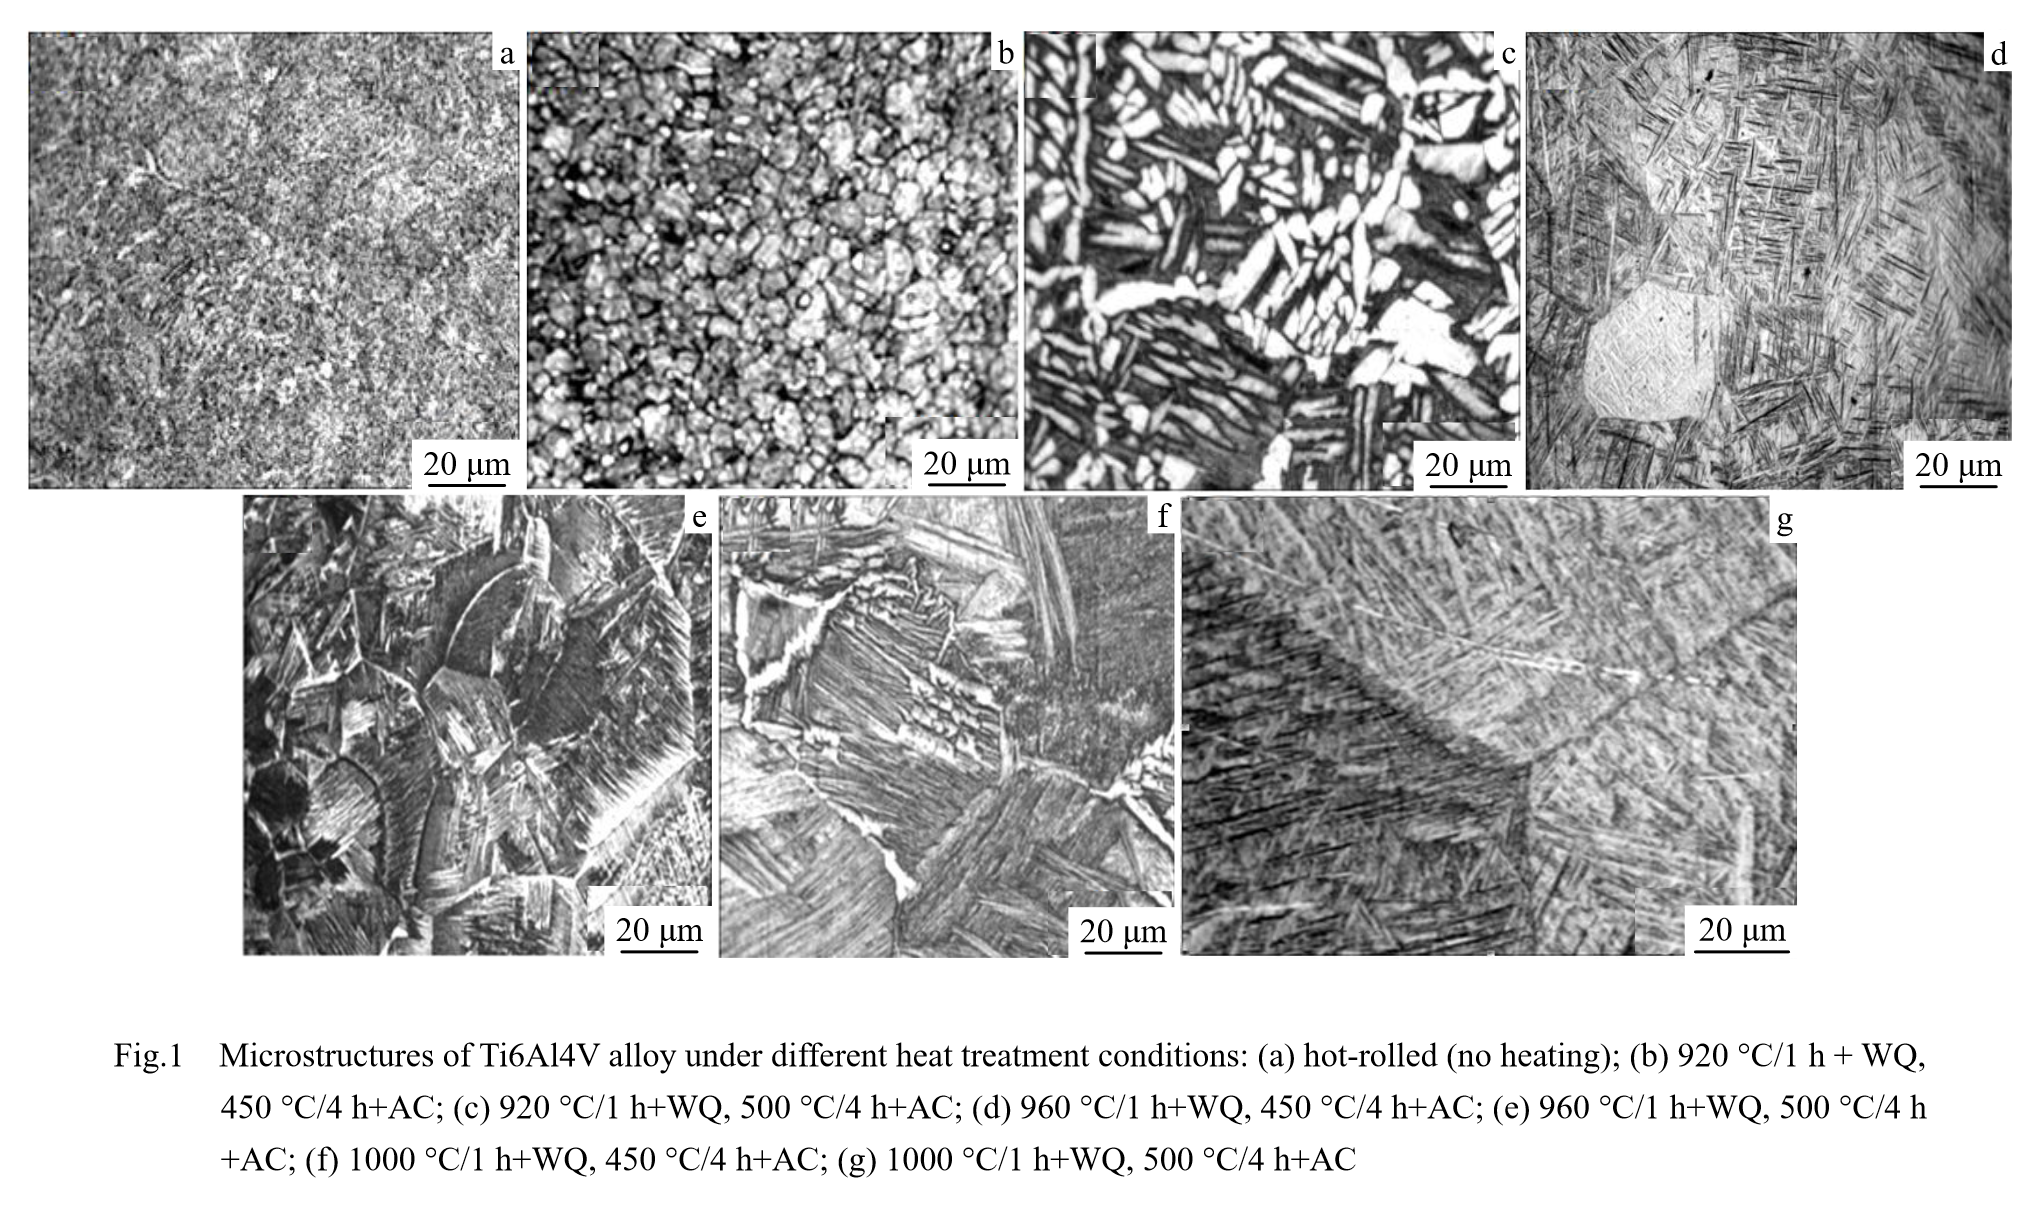
\includegraphics[width=0.8\linewidth]{金相_甲}
	\caption[参考一]{组织金相图}
	\label{fig:}
\end{figure}
% TODO: \usepackage{graphicx} required
\begin{figure}[h!]
	\centering
	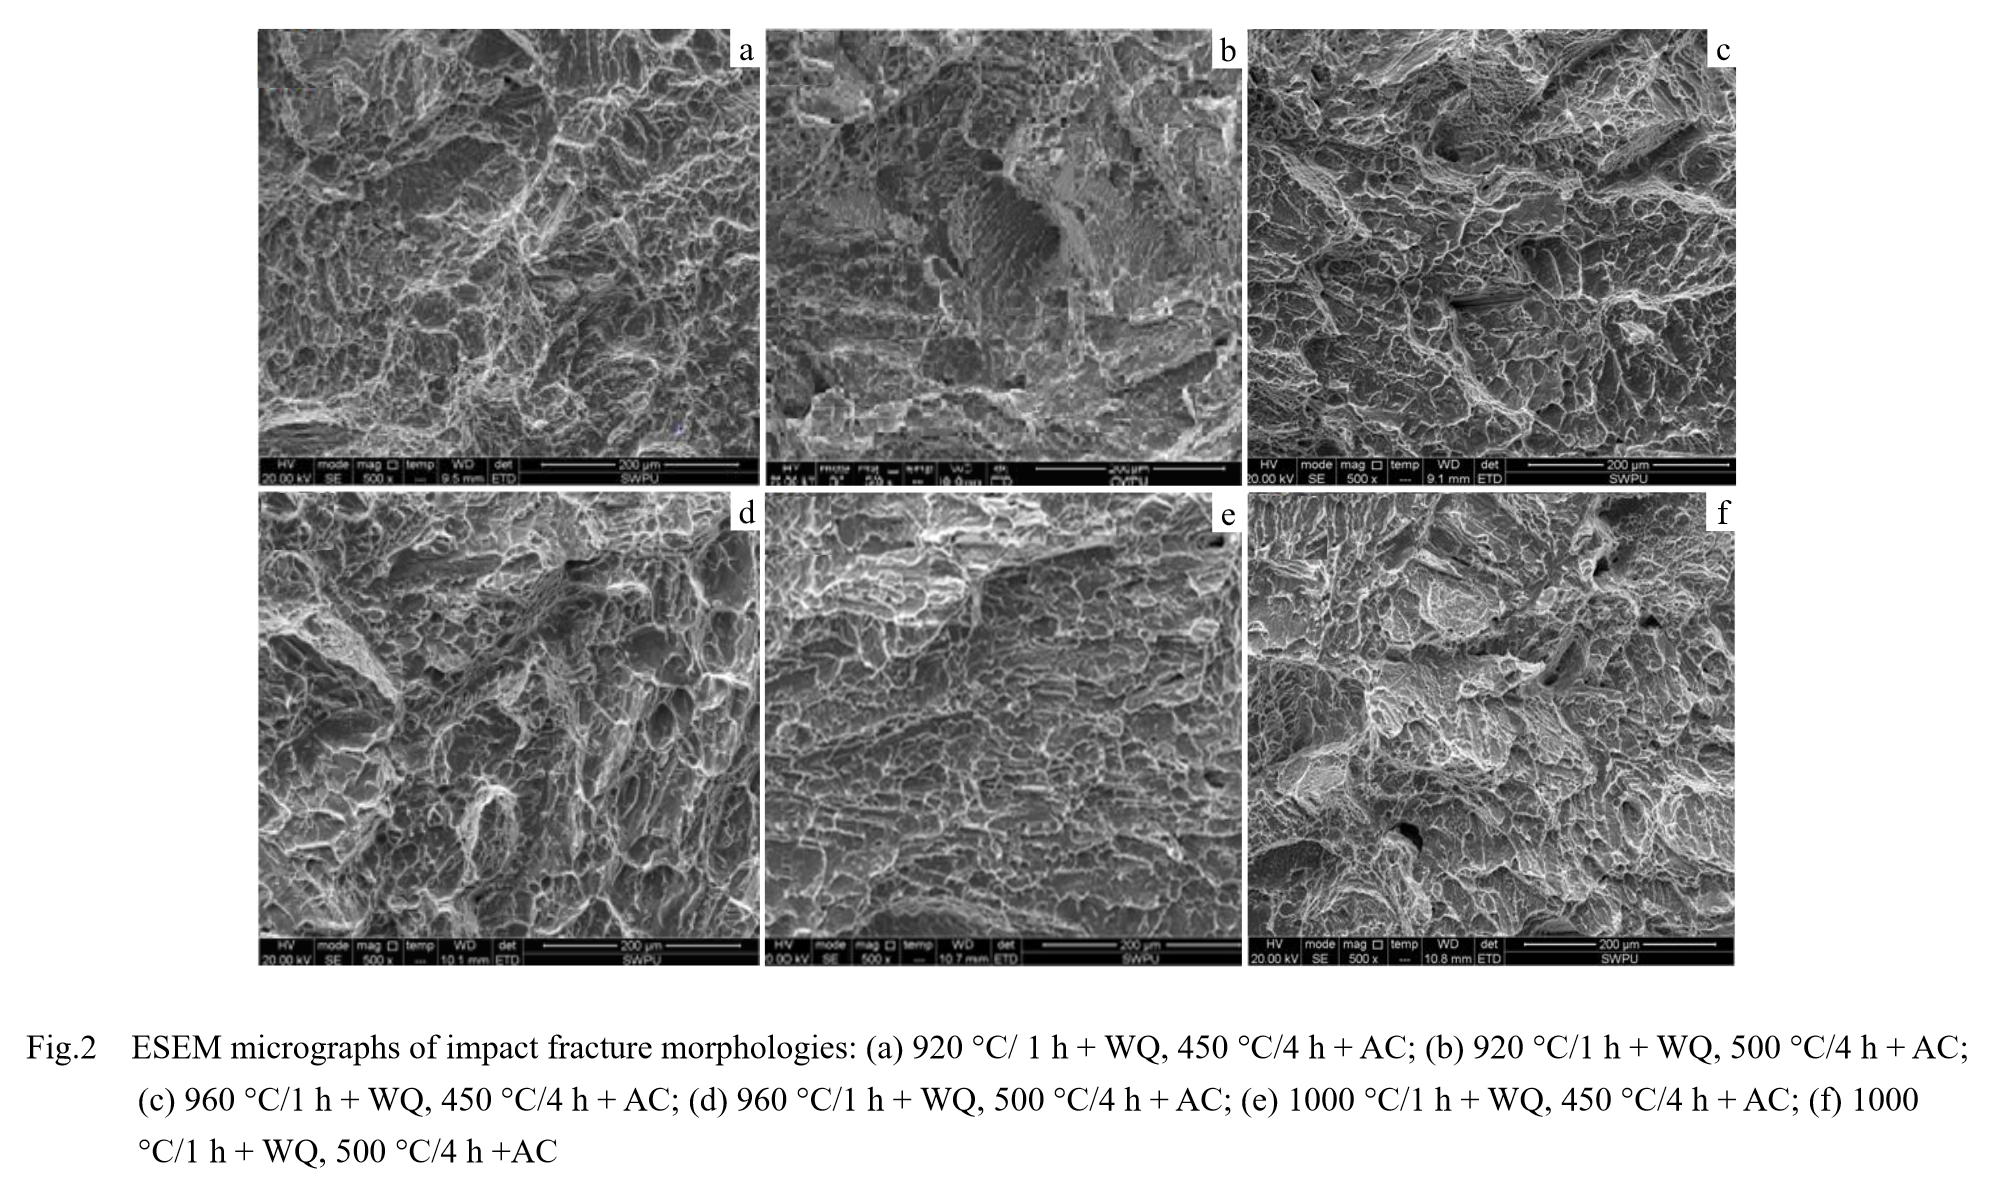
\includegraphics[width=0.8\linewidth]{其他_甲}
	\caption{断口形貌}
	\label{fig:}
\end{figure}
\section{参考乙}
	\begin{table}[htbp]
	\centering
	\label{sec:my1HT}
	\caption{\ti 热处理工艺与性能汇总表\cite{RanXingGuRongWenDuDuiTi6Al4VELITaiHeJinXianWeiZuZhiJiXingNengDeYingXiang2021}}
	\resizebox{\textwidth}{!}{
		\begin{tabular}{ccccccccc}
			\toprule
			固溶温度/℃ &用时/h & 冷却 & 时效温度/\textcelsius &用时/h & 冷却&屈强/Mpa&抗拉强度/Mpa&延伸率$\%  $\\
			\midrule
			\hot{952}{2}{WQ}{730}{4}{AC}{846}{915}{16.80}\\
			\hot{967}{2}{WQ}{730}{4}{AC}{801}{875}{11.2}\\
			\hot{997}{2}{WQ}{730}{4}{AC}{792}{861}{9.6}\\
			\hot{1012}{2}{WQ}{730}{4}{AC}{775}{843}{8.2}
			\bottomrule
		\end{tabular}
	}
\end{table}
\begin{figure}[h!]
	\centering
	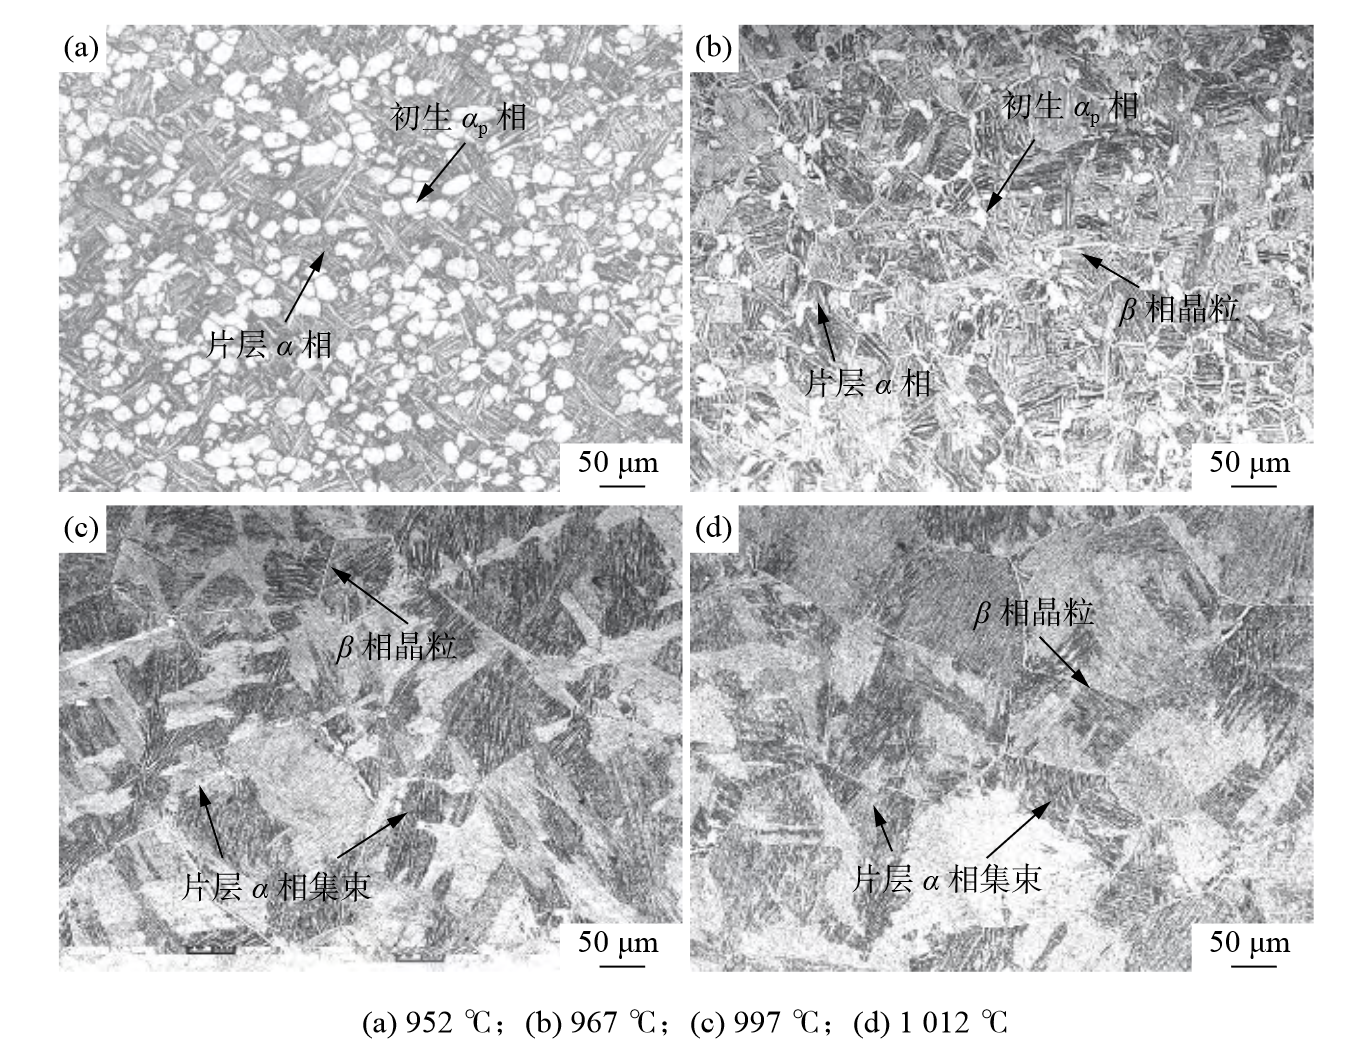
\includegraphics[width=0.7\linewidth]{金相_乙}
	\caption{金相组织}
	\label{fig:}
\end{figure}
% TODO: \usepackage{graphicx} required
\begin{figure}[h!]
	\centering
	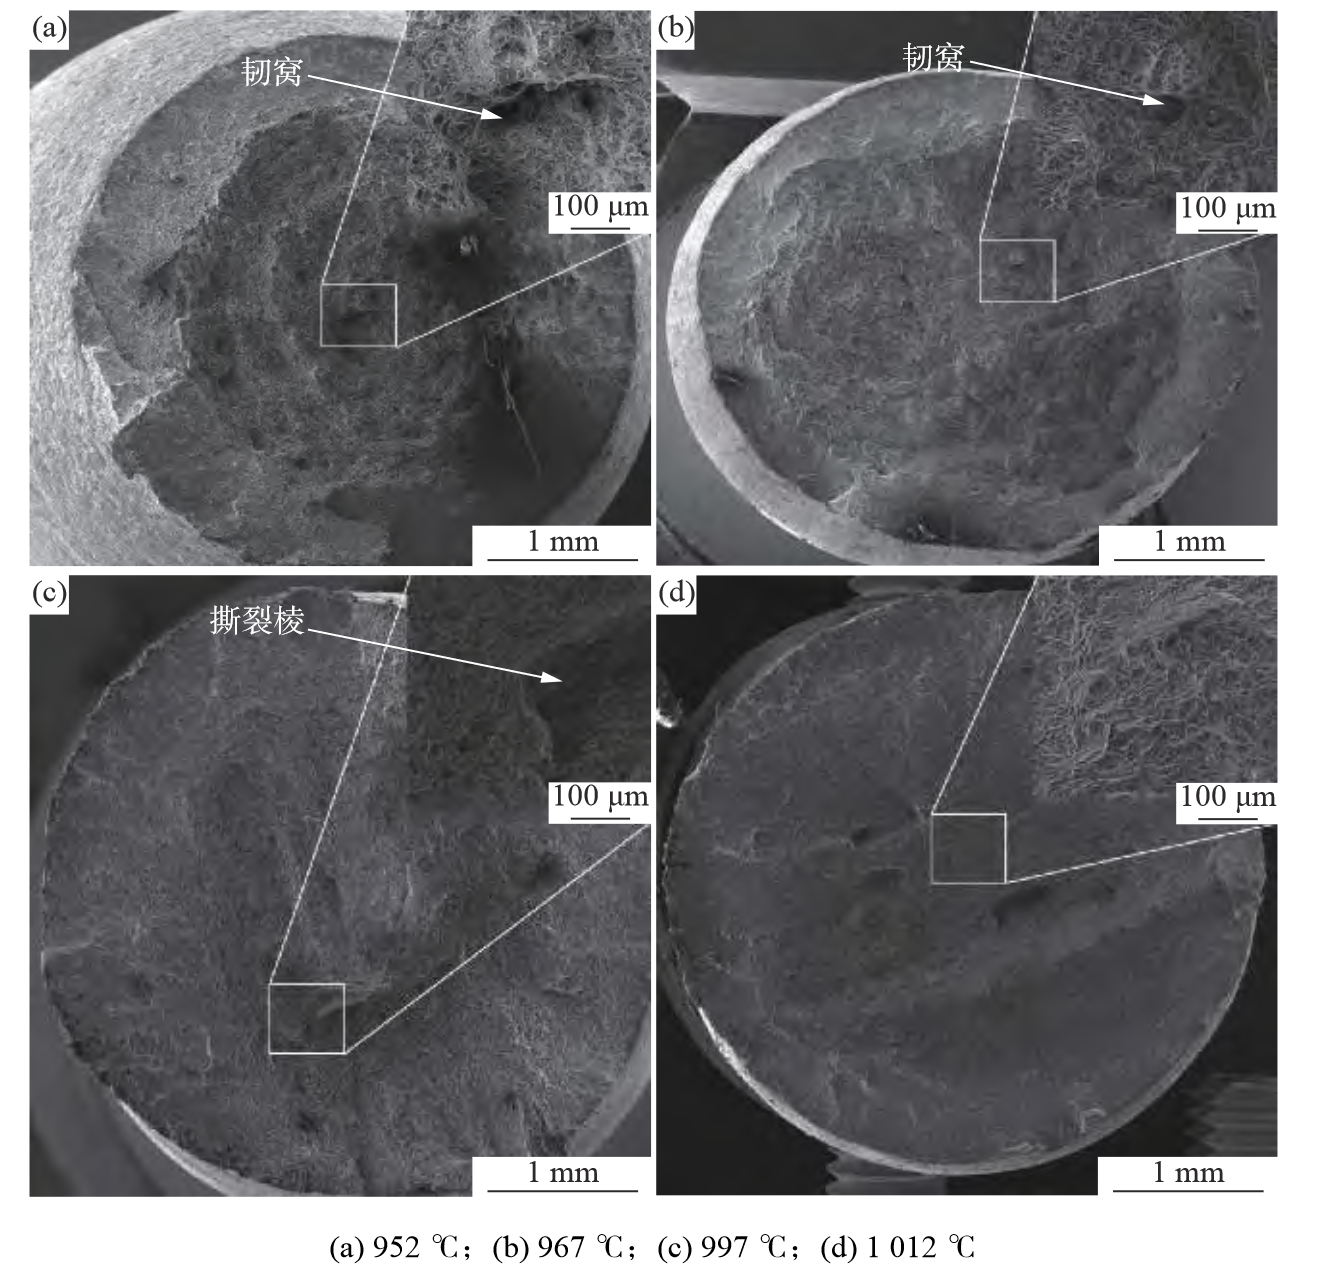
\includegraphics[width=0.7\linewidth]{断口_乙}
	\caption{断口形貌}
	\label{fig:}
\end{figure}

	\chapter{热处理工艺对显微组织转变的影响}
	\chapter{热处理工艺对力学性能的影响}

	\section{固溶温度、固溶时间}
	\section{时效温度、时效时间}
	\chapter{热处理工艺对其他性能的影响}

	\chapter{发展趋势}
	\chapter{结论}
	\begin{enumerate}
		\item 对于组织
		\item 对于力学性能
		\item 对于其他性能
	\end{enumerate}


	\backmatter
	\listoffigures
	\listoftables
	\clearpage
	\phantomsection
	\addcontentsline{toc}{chapter}{参考文献}
	\bibliography{modern}


\end{document}


